% TODO - Move this into the docs and the code. 

\chapter{Neural Networks}
\label{ch:neural}

Convolutional Neural Networks (CNN), are a kind of neural network purpose-built to process grid-like data \cite{lecun1989generalization}. CNN use convolution to handle data like image, with local connectivity. The GC-MS data is a time-series n-dimensional data. The positions of timestamps relative to each other are relevant - they share local connectivity. A peak on the graph can be considered a collection of intensities with local maxima. A CNN may learn to recognize a peak in the data - each as their distinct feature.

Still, it is a difficult task. The data is often warped due to a variety of compounding factors - such as the experimental setup \cite{tomasi2004correlation,zhang2008two}. We expect the same peak to be at different timestamps across multiple samples. A CNN can generalize. It can use techniques such as convolution \cite{lecun1989generalization} and pooling \cite{zhou1988image} to represent a feature as a peak within a given vicinity. CNN has been shown to consistently outperform other ML models in tasks related to gas-chromatograph data \cite{bi2020gc, matyushin2020gas}.

\section{Network}
\label{sec:network}

The network perfoms a classification task. It maps a given input to an output, in the form $f: X \to Y$ where $X \in \R^{d_1 \times d_2 \times d_3}$ and $Y \in \left\{ y \in \{0,1\}^n : \sum^n_{i=1} y_i = 1 \right\}$ with parameters $\theta$. For compatibility with Keras \cite{chollet2015keras} we use one-hot encodings. The model tunes its weights and biases ($\theta$) through backpropagation during training. Weights scale the impact of input on its output. Biases change when a neuron fires.

\subsection{Convolution}
\label{sec:convolution}

We have time-series GC-MS data. This data is suited towards a CNN due to their local connectivity. A group of intensities measures close to each other (i.e a resolved peak) are likely to represent a chemical compound. Convolution introduces purpose-built layers to a neural network. Layers suited towards data with local connectivity. In particular, this model introduces convolutional and pooling layers.

Convolution is a type of linear operation \cite{goodfellow2016deep}. Rather than general matrix multiplication, convolution provides a narrow receptive field. Like how we can view a solar eclipse through a pinpoint viewing hole. Convolutional layers have neurons that map to a specific region of their input.

A pooling function transforms the output of a new into summary statistics of its neighbours \cite{goodfellow2016deep}. It can tell a feature is around here, without knowing its explicit location. Max pooling returns the largest value in an area \cite{zhou1988image}. Pooling provides dimensionality reduction. We reduce the complexity at the sacrifice of the image resolution.

\subsection{Rectified Linear Unit(s)}
\label{sec:relu}

The Rectified Linear Unit (relu) is a non-linear activation function. See fig (d). First used in neural networks in the 1980s by Fukushima \cite{fukushima1982neocognitron}. Denoted mathematically below.

\[ \varphi (x) = \begin{cases}
        x & x \ge 0 \\
        0 & x < 0
    \end{cases}
\]

Without non-linearity a network becomes a linear function of its input \cite{goodfellow2016deep}. ReLU is close to linear. It maintains desirable aspects that come with optimizing linear models \cite{goodfellow2016deep}.

\subsection{Categorical Cross-Entropy}
\label{sec:categorical-cross-entropy}

The loss function for the network is Categorical Cross-Entropy (CCE). It quantifies the difference between two probability distributions. The actual $p$, and predicted $q$ output distributions. That difference is the information or the average number of bits. Line (1) shows CCE derived from the Kullback-Liebler divergence \cite{kullback1951information}. Defined mathematically below.

\begin{align}
    H(p,q) & = H(p) + D_{KL}(p||q)             \\
           & = - \sum_{x \in X} p(x) \log q(x) \\
           & = - E_p [\log q]
\end{align}

The Kullback-Liebler objective function is the same as minimizing the cross-entropy. The objective function (KL) minimizes the loss function (CCE). During training, it optimizes its parameters $\theta$ to reduce loss.

\section{Parameter Settings}

A 1D-conv net is proposed. It has a dropout layer ($p = 0.5$) for regularisation. The output layer used a softmax activation function \cite{simonyan2014very}. The rest use ReLU \cite{fukushima1982neocognitron}. The network has learning rate $\eta = 0.01$, epochs $n = 20$ and batchsize $b = 8$. The Adam \cite{kingma2014adam} optimizer  with $\beta_1 = 0.9$, $\beta_2 = 0.999$ and $\epsilon = 10^{-7}$.

\begin{table}[H]
    \caption{Architecture: CNN}
    \vspace{0.5cm}
    \centering
    \label{tab:aug_architecture}
    \begin{tabular}{lll}
        \hline
        Layer (type)                  & Output Shape     & Param \# \\ \hline
        conv1d (Conv1D)               & (None, 4800, 64) & 1344     \\
        max\_pooling1d (MaxPooling1D) & (None, 1200, 64) & 0        \\
        dropout (Dropout)             & (None, 1200, 64) & 0        \\
        flatten (Flatten)             & (None, 76800)    & 0        \\
        dense (Dense)                 & (None, 64)       & 4915264  \\
        dense\_1 (Dense)              & (None, 4)        & 260      \\ \hline
    \end{tabular}
\end{table}

\section{Experimental Results}
\label{sec:nn-results}

\begin{table}[H]\label{t:cnn-results}
    \centering
    \begin{tabular}{|l|l|l|l|l|l|l|}
        \hline
        Dataset      & AvgTrain $\pm$ Std & T & AveTest $\pm$ Std & T \\
        \hline
        Fish Species & 1 $\pm$ 1          & + & 94.09 $\pm$ 4.19  & - \\
        Fish Part    & 99.15 $\pm$ 1.04   & - & 81.02 $\pm$ 6.99  & - \\
        \hline
    \end{tabular}
    \caption{Experimental Results of CNN}
\end{table}

Table \ref{t:cnn-results} shows the performance in terms of classification accuracy for the CNN. "AveTrain $\pm$ Std" and "AveTest $\pm$ Std" show the average classification performance and their standard deviation of the experiment's 30 runs. "T" represents the statistical significance test mentioned in section \ref{s:parameter}. "+" is an improvement. "-" is worse performance. "=" is the same as the SVM. We compare the results to SVM, which is the current best performing classification algorithm.

\begin{figure}[H]
    \centering
    \begin{minipage}{.5\textwidth}
        \centering
        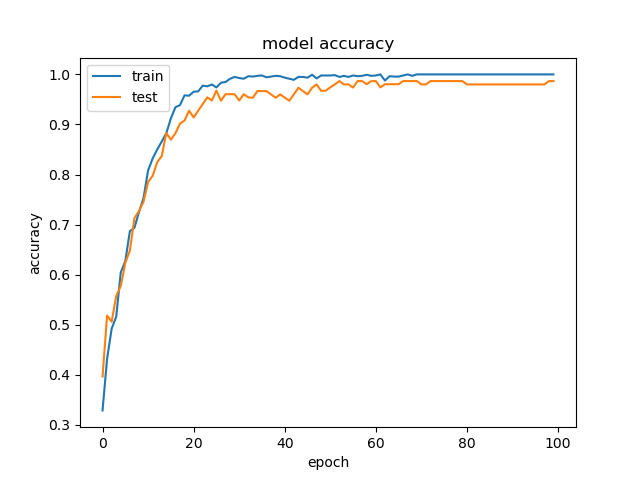
\includegraphics[width=\linewidth]{nn/fish/accuracy}
        \caption{Accuracy}
        \label{fig:FISH-cnn-acccuracy}
    \end{minipage}%
    \begin{minipage}{.5\textwidth}
        \centering
        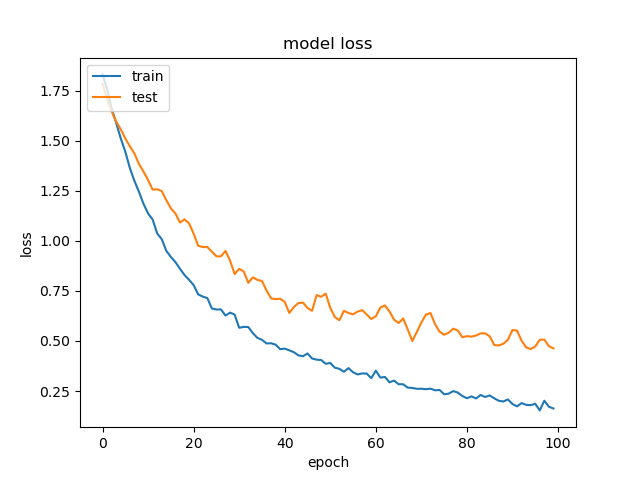
\includegraphics[width=\linewidth]{nn/fish/loss}
        \caption{Loss}
        \label{fig:FISH-cnn-loss}
    \end{minipage}
\end{figure}

Figure~\ref{fig:FISH-cnn-acccuracy} shows the classification accuracy using CNN on the fish species dataset. Figure~\ref{fig:FISH-cnn-loss} shows the classification loss using CNN on the fish species dataset. We measure the categorical cross-entropy as the loss function (\S~\ref{sec:categorical-cross-entropy}). The results show the CNN is not subject to overfitting and can generalize on unseen data.

\begin{figure}[H]
    \centering
    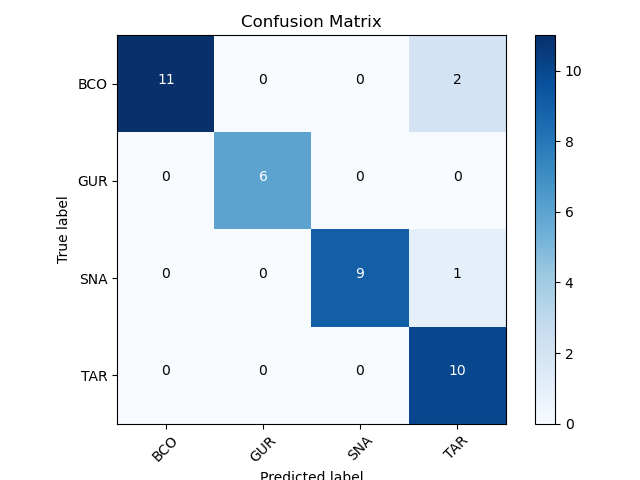
\includegraphics[width=8.5cm]{nn/fish/confusion_matrix}
    \caption{CNN: Confusion Matrix on Fish Species}
    \label{fig:FISH-cnn-confusion}
\end{figure}

Figure~\ref{fig:FISH-cnn-confusion} shows the confusion matrix for the fish species dataset using CNN. In this run, the model was able to correctly identify all but one sample from the fish species dataset.

\section{Results of CNN}

The results table \ref{t:results} shows that the CNN performance. For the fish species data, the algorithm achieves 100\% (perfect accuracy) on training and 94\% on the test. For the fish part data, the algorithm achieves 99\% (near perfect) on training and 81\% on the test. It is interesting to note that the algorithm cannot consistently fit the training data for the fish part. This suggests the dataset is more difficult to learn under the given parameters.

\section{Comparisons with SVM}

The results table \ref{t:results} compares the predictive performance for the CNN to SVM for statistical significance. Recall from chapter \ref{ch:visualization}, the performance of the SVM. For the fish species data, for the test data, the CNN gets 94.0\% which is comparable to the 99.5\% SVM. For the fish part data, on the test data the CNN has 81\% and SVM 87\%. The CNN performs worse than SVM for both datasets on unseen data.

\section{Conclusion}

The high accuracy of the SVM on the fish species was an incredible result. This classifier did not maintain this standard when classifying the fish part. A CNN is a black-box method, that can achieve high-predictive accuracy, at the expense of interpretability. We train a 1D CNN on the fish dataset to explore the learnability of the fish species dataset. We hypothesize that if it performs well on the fish species, and poorly on the fish part, this dataset may be inherently difficult to learn. Therefore perhaps, an exercise of diminishing to try improving performance on.

The results proved the initial hypothesis correct. The CNN was performant on the fish species. It achieved close, but not quite the same accuracy as the SVM for the fish part dataset. However, similar to the SVM, neither model was able to achieve higher than 87\% accuracy on the fish part dataset. This hinted - but does not prove indefinitely - that the fish part is a harder dataset to learn.

